\documentclass[a4paper,12pt]{exam}
	\usepackage{graphicx}
	\usepackage[utf8]{inputenc}
	\usepackage[T1]{fontenc}
	\usepackage{listings}
	\usepackage{color}
	\usepackage{amsmath}
	\usepackage{enumerate}
	\definecolor{dkgreen}{rgb}{0,0.6,0}
	\definecolor{gray}{rgb}{0.5,0.5,0.5}
	\definecolor{mauve}{rgb}{0.58,0,0.82}

	\lstset{frame=tb,
	  language=Python,
	  aboveskip=3mm,
	  belowskip=3mm,
	  showstringspaces=false,
	  columns=flexible,
	  basicstyle={\small\ttfamily},
	  numbers=none,
	  numberstyle=\tiny\color{gray},
	  keywordstyle=\color{blue},
	  commentstyle=\color{dkgreen},
	  stringstyle=\color{mauve},
	  breaklines=true,
	  breakatwhitespace=true
	  tabsize=3
	}

\begin{document}
	\begingroup 
	  \bf Mecânica Clássica I - Resolução do exercício 3 da primeira prova\\
	  \indent André Del Bianco Giuffrida
	\endgroup
	\\ 
	\\ 
	\indent \textit{ Uma partícula de massa $m$ está sujeita a uma força:}
		$ \vec{F}(r)= -\frac{\beta}{r^3}\hat{r} $ \textit{ onde $\beta$ é uma constante positiva.}
		\indent Sabemos que para uma força conservativa $\vec{F}(r)= - \nabla V(r)$ e para verificar se F é conservativa basta verificar se: $\nabla \times \vec{F}(r) = 0$, isso é característico de uma força central e como segue vemos que :
		\[ \nabla \times \vec{F}(r) = \frac{1}{r^2 sin(\theta)}
			\begin{vmatrix}
				\hat{r} & r \hat{\theta} & rsin(\theta)\hat{\varphi} \\
				\frac{\partial}{\partial r} & \frac{\partial}{\partial \theta} & \frac{\partial}{\partial \varphi} \\
				\vec{F_r}(r) & 0 & 0 
			\end{vmatrix}
		= \frac{\partial}{\partial \varphi} \frac{\vec{F_r}(r)}{r sin(\theta)}\hat{\theta} -  \frac{\partial}{\partial \theta} \frac{\vec{F_r}(r)}{r} \hat{\varphi} = 0
		\] 
		\[ \text{Com isso: \quad \quad} V(\infty) - V(r) = - \int_{r}^{\infty} F(r')dr' = \int_{r}^{\infty} \frac{\beta}{r'^3} dr' = -\frac{\beta}{2r'^2} \Bigg|_{r}^{\infty} = +\frac{\beta}{2r^2}\]
		Como $V(\infty) = 0$ obtemos que o potencial da força é dado por $ V(r) = -\frac{\beta}{2r^2} $
		\\
		Uma vez que: $E = T + V$ onde, a princípio $T = \frac{mv^2}{2} + \frac{mr^2\dot\theta^2}{2}$, se a partícula está restrita ao plano horizontal, não existe variação do momento angular , ou seja, $L = m r^2 \dot\theta$ é uma constante de modo que, podemos interpretar o termo $\frac{mr^2\dot\theta^2}{2}$ como uma energia potencial, obtendo $E = \frac{mv^2}{2} + \big[\frac{ L^2 }{2mr^2} + V(r) \big]$ e assim obtendo o potencial efetivo:
		\[ V_{ef} = \frac{ L^2 }{2mr^2} - \frac{\beta}{2r^2}  = \frac{1}{2r^2} \Bigg[\frac{L^2}{m} - \beta \Bigg] \]
		
		Partindo de $\vec{F} = m\vec{a}$ temos $-\frac{\beta}{r^3}\hat{r} = m \big(\ddot{r} - r\dot{\theta}^2 \big)\hat{r} $ , ou seja, $ \ddot{r} - \frac{L^2}{m^2 r^3} = -\frac{\beta}{mr^3}$ com isso obtemos a seguinte equação:
		
		\[ m\ddot{r} = \frac{L^2}{mr^3} - \frac{\beta}{r^3} \]
		Para resolver essa EDO vamos fazer uma mudança de variável e vamos usar a regra da cadeia. de modo que:
		\[\frac{dr}{dt} = \frac{dr}{d\theta}\frac{d\theta}{dt} \]
		e assim \[\frac{dr}{dt} = \frac{dr}{d\theta}\dot{\theta} \]
		Usando a conservação do momento angular, 
		\[ \frac{dr}{dt} = \frac{dr}{d\theta}\frac{L}{mr^2} \] 
		
		
		\[ \frac{L}{r^2}\frac{d}{d\theta} \Big[ \frac{L}{mr^2} \frac{dr}{d\theta} \Big] = \frac{L^2}{mr^3} - \frac{\beta}{r^3} \]
		\[ \frac{L^2}{mr^2}\frac{d}{d\theta} \Big[ \frac{1}{r^2} \frac{dr}{d\theta} \Big]  = \frac{L^2}{mr^3} - \frac{\beta}{r^3} \]
		
		\[ \frac{L^2}{mr^2} \Big[ \frac{-2}{r^3} \Big(\frac{dr}{d\theta}\Big)^2 + \frac{1}{r^2} \frac{d^2r}{d\theta^2} \Big] = \frac{L^2}{mr^3} - \frac{\beta}{r^3} \]
		afim de simplificar fazemos
		\[\frac{1}{r} = u \]
		obtemos derivando
		\[\frac{du}{d\theta} = -\frac{1}{r^2}\frac{dr}{d\theta}  \]
		\[\frac{d^2u}{d\theta^2} = \frac{2}{r^3} \big(\frac{dr}{d\theta}\Big)^2 - \frac{1}{r^2}\frac{d^2r}{d\theta^2}  \]
		
		agora substituindo ficamos com:
		
		\[ -\frac{L^2}{mr^2} \frac{d^2u}{d\theta^2} = \frac{L^2}{mr^3} - \frac{\beta}{r^3} \]
		
		\[ -\frac{L^2}{m} \frac{d^2u}{d\theta^2} = \frac{L^2 u}{m} - \frac{\beta u}{1} \]
		\[ -\frac{d^2u}{d\theta^2} = u - u\frac{\beta m}{L^2} \]
		
		\[ \frac{d^2u}{d\theta^2} = u \Big( \frac{\beta m}{L^2} -1 \Big) \]
		
		\[ \frac{d^2u}{d\theta^2} + u \Big( 1- \frac{\beta m}{L^2} \Big) = 0 \]
		
		a solução aqui fica \[ u(\theta) = Acos(\omega \theta - \varphi) \]
		onde $\omega = sqrt(\frac{\beta m}{L^2} - 1 )$
		e assim temos que
		\[ r(\theta) = \frac{1}{Acos(\omega \theta - \varphi)}\]
		Onde $\omega = sqrt(1- \frac{\beta m}{L^2}$)
		
		%Possíveis condições iniciais:
		%\[\left\{ 
		%	\begin{array}{l l}
		%		L^2 = \beta m \\ L^2 < \beta m \\ L^2 > \beta m \\
		%	\end{array} 
		% \right.
  		%\]
		
		\begin{figure}[l]
			\centering
			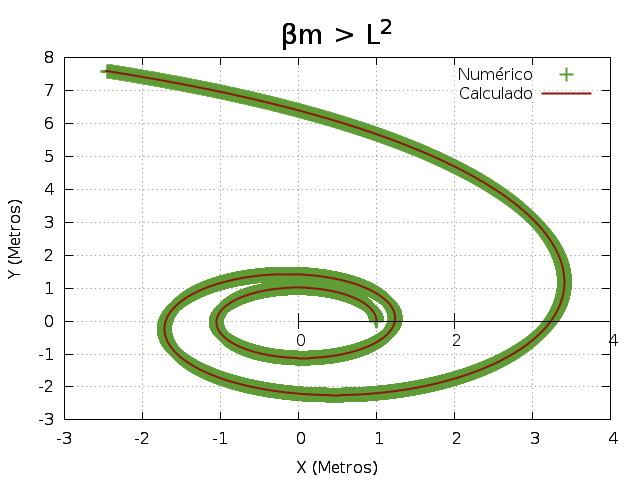
\includegraphics[scale=0.3]{3o0.png}
			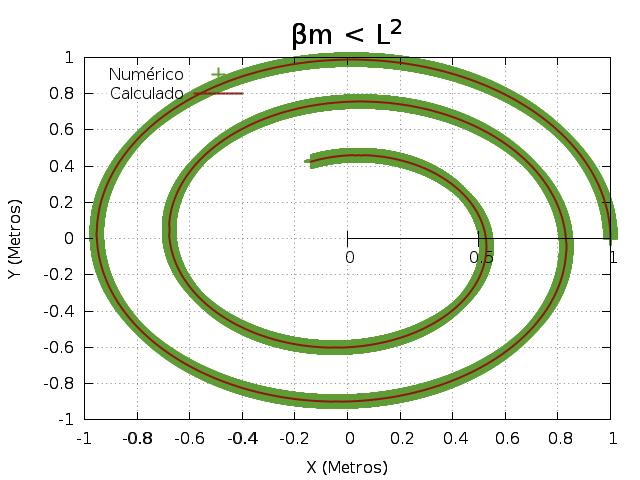
\includegraphics[scale=0.3]{3o1.png}
			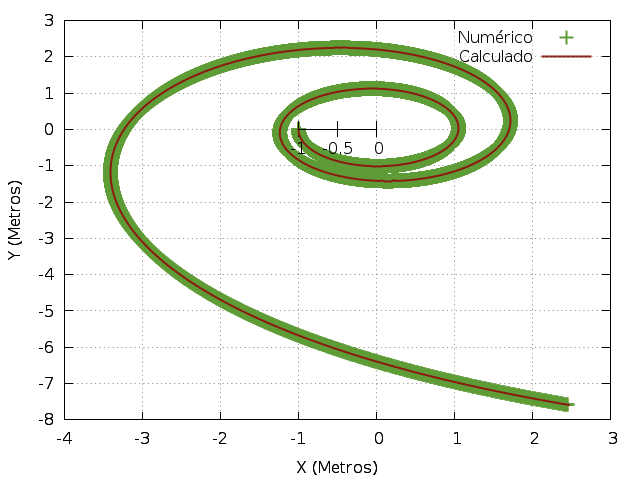
\includegraphics[scale=0.3]{3o2.png}
			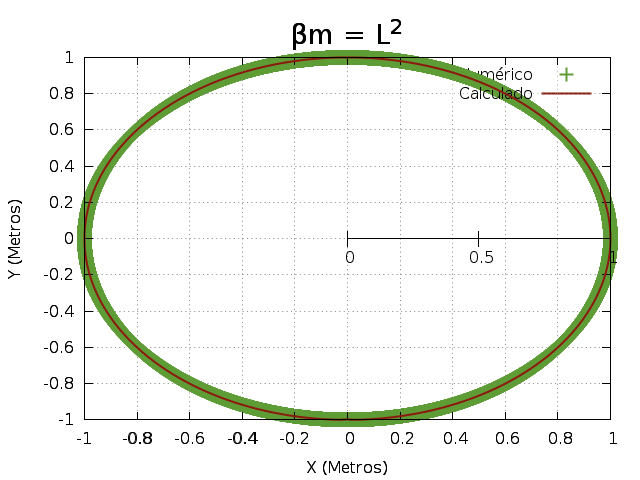
\includegraphics[scale=0.3]{3o3.png}
			
		\end{figure}
	\end{document}
